%&pdflatex
\documentclass[mathserif]{beamer} %, handout
\usetheme[progressbar=foot]{metropolis}
\setbeamertemplate{caption}[numbered]

\usepackage[utf8x]{inputenc}
\usepackage[T2A]{fontenc}
\usepackage[english,russian]{babel}

\usepackage{amssymb, amsmath, amsfonts, mathtools, mathrsfs}
\usepackage{comment}

\AtBeginSubsection{
\frame[plain,c]{\subsectionpage}
}

\defbeamertemplate{subsection page}{simple}{
  \centering
  \usebeamercolor[fg]{subsection title}
  \usebeamerfont{subsection title}
  \insertsubsection\\
}
\setbeamertemplate{subsection page}[simple]

\title{Численный и асимптотический анализ уравнения Больцмана.\\ Некоторые классические задачи молекулярной газодинамики}
\author{Рогозин Олег Анатольевич}
\institute{
    Московский физико-технический институт (ГУ) \\
    Вычислительный центр ФИЦ ИУ РАН
}
\date{\today}

\newcommand{\Kn}{\mathrm{Kn}}
\newcommand{\Ma}{\mathrm{Ma}}
\newcommand{\dd}{\:\mathrm{d}}
\newcommand{\pder}[2][]{\frac{\partial#1}{\partial#2}}
\newcommand{\pderdual}[2][]{\frac{\partial^2#1}{\partial#2^2}}
\newcommand{\pderder}[2][]{\frac{\partial^2 #1}{\partial #2^2}}
\newcommand{\Pder}[2][]{\partial#1/\partial#2}
\newcommand{\dzeta}{\boldsymbol{\dd\zeta}}
\newcommand{\bzeta}{\boldsymbol{\zeta}}
\newcommand{\bh}{\boldsymbol{h}}
\newcommand{\be}{\boldsymbol{e}}
\newcommand{\Nu}{\mathcal{N}}
\newcommand{\OO}[1]{O(#1)}
\newcommand{\Set}[2]{\{\,{#1}:{#2}\,\}}
\newcommand{\deltann}[2]{(\delta_{#1#2}-n_#1 n_#2)}
\newcommand{\onwall}[1]{\left(#1\right)_0}
\newcommand{\xoverbrace}[2][\vphantom{\int}]{\overbrace{#1#2}}

\begin{document}

\frame{\titlepage}

\begin{frame}
  \frametitle{Содержание}
  \linespread{0.8}
  \tableofcontents
\end{frame}

\section{Численный анализ}

\subsection{Метод решения уравнения Больцмана}

\begin{frame}
    \frametitle{Расщепление уравнения Больцмана}
    \vspace{-5pt}
    \begin{equation}
        \pder[f]{t} + \zeta_i\pder[f]{x_i} = J(f,f)
    \end{equation}
    \pause\vspace{-10pt}
    \begin{block}{Симметричная схема расщепления}
        \begin{equation}
            S_{A+B}^{\tau} = S_A^{\tau/2}S_B^{\tau}S_A^{\tau/2} + \OO{\tau^2}
        \end{equation}
        \centering [Strang 1968; Bobylev, Ohwada 2001]
    \end{block}
    \vspace{-10pt}
    \begin{columns}[T]
        \pause
        \begin{column}{5cm}
            \begin{block}{Бесстолкновительное УБ}
                \begin{equation}
                    \pder[f]{t} + \zeta_i\pder[f]{x_i} = 0
                \end{equation}
                \vspace{-15pt}
                \begin{itemize}
                    \item метод конечных объёмов
                    \item TVD-схема \(\OO{\tau^2, h^2}\)
                    \item сетка с помощью GMSH
                \end{itemize}
            \end{block}
        \end{column}
        \pause
        \begin{column}{6.5cm}
            \begin{block}{Пространственно-однородное УБ}
                \begin{equation}
                    \pder[f]{t} = J(f,f)
                \end{equation}
                \vspace{-15pt}
                \begin{itemize}
                    \item проекционный метод дискретных скоростей
                    \item схема в дробных шагах \(\OO{\tau^2, h^2}\)
                    \item прямоугольная сетка
                \end{itemize}
            \end{block}
        \end{column}
    \end{columns}
\end{frame}

\begin{frame}
    \frametitle{Дискретизация пространства скоростей}
    Сетка \(\mathcal{V} = \Set{\zeta_\gamma}{\gamma\in\Gamma}\) построена так, что
    \begin{equation}\label{eq:zeta_cubature}
        \int F(\bzeta) \dzeta \approx \sum_{\gamma\in\Gamma} F_\gamma w_\gamma =
            \sum_{\gamma\in\Gamma} \hat{F_\gamma},
            \quad F_\gamma = F(\bzeta_\gamma),
    \end{equation}\vspace{-10pt}

    где \(\sum_{\gamma\in\Gamma} w_\gamma = V_\Gamma\) "--- объём, покрываемый скоростной сеткой.
    \pause\vspace{20pt}

    Симметризированный интеграл столкновений\vspace{-20pt}

    \begin{equation}\label{eq:symm_ci}
        J(f_\gamma, f_\gamma) = \frac14\int \left(
            \delta_\gamma + \delta_{\gamma*} - \delta'_\gamma - \delta'_{\gamma*}
        \right) (f'f'_* - ff_*)B \dd\Omega(\boldsymbol{\alpha}) \dzeta\dzeta_*
    \end{equation}\vspace{-30pt}

    имеет следующий дискретный аналог:
    \begin{equation}\label{eq:discrete_symm_ci}
        \footnotesize
        \hat{J}_\gamma = \frac{\pi V_\Gamma^2}{\displaystyle\sum_{\nu\in\Nu} w_{\alpha}w_{\beta}}
            \sum_{\nu\in\Nu} \left(
                \delta_{\alpha\gamma} + \delta_{\beta\gamma} - \alert{\delta_{\alpha'\gamma}} - \alert{\delta_{\beta'\gamma}}
            \right)\left(
                \frac{w_{\alpha}w_{\beta}}{\alert{w_{\alpha'}w_{\beta'}}}
                \alert{\hat{f}_{\alpha'}\hat{f}_{\beta'}} - \hat{f}_{\alpha}\hat{f}_{\beta}
            \right)B_\nu.
    \end{equation}\vspace{-10pt}
\end{frame}

\begin{frame}
    \frametitle{Консервативное проецирование частиц}
    Проекционный метод Петрова"--~Галёркина:
    \begin{equation}\label{eq:Petrov-Galerkin}
        \int \xoverbrace{ \psi_s(\bzeta_\gamma) }^\text{test space} \bigg(
            \delta(\bzeta'-\bzeta_\gamma) - \sum_{a\in\Lambda} r_{\lambda,a}
            \xoverbrace{ \delta(\bzeta_{\lambda+s_a}-\bzeta_\gamma) }^\text{trial space}
        \bigg) \dzeta_\gamma = 0.
    \end{equation}
    \begin{itemize}
        \item \(r_{\lambda,a}\) "--- проекционные веса (в пространстве \(\mathcal{V}\))
        \item \(\mathcal{S} = \Set{s_a}{a\in\Lambda}\) "--- проекционный шаблон \\(набор правил смещения)
        \item \(\psi_0 = 1, \psi_i = \zeta_i, \psi_4 = \zeta_i^2\) "--- столкновительные инварианты
    \end{itemize}
\end{frame}

\begin{frame}
    \frametitle{Интерполирование функции распределения}
    Среднее взвешенное по Колмогорову:
    \begin{equation}\label{eq:Kolmogorov_mean}
        \begin{dcases}
            \hat{f}_{\alpha'} = \phi^{-1}_f\left(\sum_{a\in\Lambda} q_{\lambda,a}
                \phi_f\left(\hat{f}_{\lambda+s_a}\right)\right), \\
            w_{\alpha'} = \phi^{-1}_w\left(\sum_{a\in\Lambda} p_{\lambda,a}
                \phi_w\left(w_{\lambda+s_a}\right)\right), \\
        \end{dcases}
    \end{equation}
    Если
    \begin{equation}\label{eq:geometric_mean}
       \phi_{f,w}(x) = \ln(x), \quad \phi_{f,w}^{-1}(x) = \exp(x), \quad p_{\lambda,a} = q_{\lambda,a} = r_{\lambda,a},
    \end{equation}
    то
    \begin{equation}\label{eq:strict_interpolation}
        \hat{J}_\gamma(\hat{f}_{M\gamma}, \hat{f}_{M\gamma}) = 0.
    \end{equation}
\end{frame}

\begin{frame}
    \frametitle{Задача Коши}
    Интегрируя уравнение Больцмана вдоль интервала времени~\(\tau = t_{n+1} - t_n\), получаем
    \begin{equation}\label{eq:time_scheme}
        \hat{f}_\gamma(t_{n+1}) = \hat{f}_\gamma(t_n) + \int_{t_n}^{t_{n+1}} \hat{J}(f_\gamma, f_\gamma) \dd{t},
        \quad n\ge0.
    \end{equation}
    Если переписать \(\hat{J}_{\gamma} = \sum_{j=1}^N \hat{\Delta}_{\gamma}^{n+(j-1)/N}\), где \(N=|\Nu|\), и
    \begin{equation}\label{eq:discrete_short_ci}
        \int_{(n+(j-1)/N)\tau}^{(n+j/N)\tau}\hat{J}_\gamma\dd{t} \approx
            \frac{\tau}{N} \hat{\Delta}_{\gamma}^{n+(j-1)/N},
    \end{equation}
    \pause
    то получается обеспечивающая \(\hat{f}_\gamma^n = \hat{f}_\gamma(t_0) + \OO{\tau^2}\)
    \begin{block}{схема в дробных шагах}
        \vspace{-5pt}
        \begin{equation}\label{eq:fractional_step_scheme}
            \hat{f}_\gamma^{n+j/N} = \hat{f}_\gamma^{n+(j-1)/N} + \frac{\tau}{N}\hat{\Delta}_{\gamma}^{n+(j-1)/N}
            \quad (j = 1,\dotsc,N).
        \end{equation}
        \vspace{-10pt}
    \end{block}
\end{frame}

\begin{frame}
    \frametitle{Положительность функции распределения}
    \begin{block}{}
        \vspace{-5pt}
        \begin{equation}\label{eq:positive_f}
            \hat{f}_\gamma^{n+j/N} > 0 \implies \alert{ \forall \gamma\in\Gamma, \forall\nu\in\Nu\!: \
                \hat{f}_\gamma + \frac{\tau}{N}\hat{\Delta}_{\gamma\nu} > 0 }
        \end{equation}
        \vspace{-10pt}
    \end{block}
    \vspace{20pt}\pause

    Если \(\gamma = \alpha\), то получаем оценку
    \begin{equation}\label{eq:positive_f_alpha}
        \alert{ |\Nu| > \hat{A} \hat{f}_{\max} }, \quad
        \hat{A} = \pi\frac{\tau V_\gamma|\Nu| B_{\max}}{\sum_{\nu\in\Nu} w_{\alpha}w_{\beta}}
    \end{equation}
    где
    \begin{equation}\label{eq:hat_f_max}
        \hat{f}_{\max} = \max_{\gamma\in\Gamma} \hat{f}_\gamma, \quad
        B_{\max} = \max_{\boldsymbol\alpha, \bzeta, \bzeta_*} B.
    \end{equation}
    Для модели твёрдых сфер
    \begin{equation}\label{eq:B_HS}
        B = \frac{|\boldsymbol\alpha\cdot(\bzeta_*-\bzeta)|}{4\sqrt{2\pi}} \leq \frac{\zeta_{\max}}{2\sqrt{2\pi}}.
    \end{equation}
\end{frame}

\begin{frame}
    \frametitle{Положительность функции распределения}
    Для рассмотрения \(\gamma = \lambda+s_a\) дополнительно предположим
    \begin{equation}\label{eq:normal_stencil}
        r_{\lambda,a} \leq 1, \quad q_{\lambda,a} \leq 1.
    \end{equation}
    Если \(r_{\lambda,a} \geq 0\), то
    \begin{equation}\label{eq:positive_f_lambda2+}
        |\Nu| > \hat{A} \hat{f}_{\max} \alert{ \epsilon_f^2 \epsilon_w^2 },
    \end{equation}
    Если \(r_{\lambda,a} < 0\), то
    \begin{equation}\label{eq:positive_f_lambda2-}
        |\Nu| > \hat{A} \hat{f}_{\max} \epsilon_f^2 \epsilon_w^2 \alert{
            \max_{a\in\Lambda,\gamma\in\Gamma}\left(-r_{\gamma,a}\right)
            \max_{\bzeta_\alpha,\bzeta_\beta\in\mathbb{R}^3}
            \frac{f_{\alpha}f_{\beta}}{f_{\alpha'}f_{\beta'}}
        }.
    \end{equation}
    Оценка~\eqref{eq:positive_f_lambda2-} минимальна для распределения Максвелла, когда
    \begin{equation}
        f_{\alpha}f_{\beta} = f_{\alpha'}f_{\beta'}.
    \end{equation}
\end{frame}

\begin{frame}
    \frametitle{Положительность функции распределения}
    Наибольшее изменение функции распределения на проекционном шаблоне
    \begin{equation}\label{eq:epsilon_f}
        \epsilon_f = \max_{\substack{s_a,s_b\in\mathcal{S}\\\gamma\in\Gamma}} \frac{\hat{f}_{\gamma+s_a}}{\hat{f}_{\gamma+s_b}}.
    \end{equation}
    Для гладкой функции распределения \(\epsilon_f\) меньше для шаблонов с меньшим \emph{диаметром}
    \begin{equation}\label{eq:stencil_diameter}
        R_\mathcal{S} = \max_{\substack{s_a,s_b\in\mathcal{S}\\\gamma\in\Gamma}}
            \left| \bzeta_{\gamma+s_a} - \bzeta_{\gamma+s_b} \right|.
    \end{equation}
    Максимальное отношение весов скоростной сетки
    \begin{equation}\label{eq:epsilon_w}
        \epsilon_w = \max_{\gamma,\varsigma\in\Gamma} \frac{w_\gamma}{w_\varsigma}.
    \end{equation}
\end{frame}

\begin{frame}
    \frametitle{Исключаемые кубатурные точки}
    На практике
    \begin{equation}\label{eq:discrete_short_ci_discarded}
        \hat{J}_\gamma = \sum_{\nu\in\Nu\setminus\mathcal{M}} \hat{\Delta}_{\gamma\nu},
    \end{equation}
    где \(\mathcal{M}\) "--- множество кубатурных точек, исключённых из \(\Nu\).
    \vspace{20pt}\pause

    Достаточно поддерживать малость
    \begin{equation}\label{eq:excluded_contribution}
        \frac{\sum_{\nu\in\mathcal{M}} \left| \hat{\Delta}_{\alpha\nu} \right|}
            {\sum_{\nu\in\Nu\setminus\mathcal{M}} \left| \hat{\Delta}_{\alpha\nu} \right|}.
    \end{equation}
\end{frame}

\subsection{Примеры проекционных шаблонов}

\begin{frame}
    \frametitle{Двухточечная схема для равномерной сетки}
    \begin{equation}\label{eq:discrete_symm_ci_uniform}
        J_\gamma = \frac{\pi V_\Gamma|\Gamma|}{|\Nu|}
            \sum_{\nu\in\Nu} \left(
                \delta_{\alpha\gamma} + \delta_{\beta\gamma}
                - \delta_{\alpha'\gamma} - \delta_{\beta'\gamma}
            \right)\left( f_{\alpha'} f_{\beta'} - f_{\alpha} f_{\beta} \right)B_\nu.
    \end{equation}
    \vspace{-20pt}\pause

    Ввиду симметричности сетки, достаточно двух узлов:
    \begin{equation}\label{eq:uniform_projection}
        \delta_{\alpha'\gamma} = (1-r)\delta_{\lambda\gamma} + r\delta_{\lambda\alert{+s},\gamma}, \quad
        \delta_{\beta'\gamma} = (1-r)\delta_{\mu\gamma} + r\delta_{\mu\alert{-s},\gamma},
    \end{equation}
    где
    \begin{equation}\label{eq:r_uniform}
        r = \frac{E_0-E_1}{E_2-E_1}, \quad
        E_0 = \bzeta_{\alpha'}^2 + \bzeta_{\beta'}^2, \quad
        E_1 = \bzeta_{\lambda}^2 + \bzeta_{\mu}^2, \quad
        E_2 = \bzeta_{\lambda+s}^2 + \bzeta_{\mu-s}^2.
    \end{equation}
    \vspace{-20pt}\pause

    При этом справедливо неравенство \(0\leq r < 1\).

    Оценка на минимальное количество кубатурных точек
    \begin{equation}\label{eq:positive_f_uniform}
       |\Nu| > A f_{\max} \epsilon_f^2, \quad A = \pi \tau V_\Gamma B_{\max}.
    \end{equation}
\end{frame}

\begin{frame}
    \frametitle{Пятиточечная схема для неравномерной сетки}
    \begin{equation}\label{eq:eta_definition}
        \boldsymbol{\eta} = \bzeta_{\alpha'} - \bzeta_{\lambda}, \quad
        0 \leq \frac{\eta_i}{h^+_i} \leq \frac12, \quad
        -\frac12 \leq \frac{\eta_i}{h^-_i} \leq 0.
    \end{equation}\pause

    \emph{Компактная 5-точечная схема} строится на узлах
    \begin{equation}\label{eq:stencil_nodes_5}
        \bzeta_{\lambda+s_0} = \bzeta_{\lambda}, \quad
        \bzeta_{\lambda+s_i} = \bzeta_{\lambda} + (\bh^+\cdot \be_i)\be_i, \quad
        \bzeta_{\lambda+s_4} = \bzeta_{\lambda} + \bh^-.
    \end{equation}

    Проекционные веса вычисляются как
    \begin{equation}\label{eq:stencil_weights_5}
        r_{\lambda,0} = 1 - \sum_{j=1}^4 r_{\lambda,j}, \quad
        r_{\lambda,i} = \frac{\eta_i - r_{\lambda,4}h^-_i}{h^+_i}, \quad
        r_{\lambda,4} = \frac{\boldsymbol{\eta}\cdot(\boldsymbol{\eta} - \bh^+)}
            {\bh^-\cdot(\bh^- - \bh^+)}.
    \end{equation}
    \vspace{-20pt}\pause

    Для равномерной сетки справедливы оценки
    \begin{equation}\label{eq:weights_ranges_5}
        0 \leq r_{\lambda,0} \leq 1, \quad
        -\frac1{12} \leq r_{\lambda,i} \leq \frac{11}{24}, \quad
        -\frac18 \leq r_{\lambda,4} \leq 0, \quad
        R_\mathcal{S} = \sqrt{6}.
    \end{equation}
\end{frame}

\begin{frame}
    \frametitle{Семиточечная схема для неравномерной сетки}
    \emph{Симметричная 7-точечная схема} строится на узлах
    \begin{equation}\label{eq:stencil_nodes_7}
        \bzeta_{\lambda+s_0} = \bzeta_{\lambda}, \quad
        \bzeta_{\lambda+s_{\pm i}} = \bzeta_{\lambda} + (\bh^\pm\cdot \be_i)\be_i.
    \end{equation}

    Проекционные веса вычисляются как
    \begin{equation}\label{eq:stencil_weights_7}
        r_{\lambda,0} = 1 - \sum_{j=1}^3 r_{\lambda,j} + r_{\lambda,-j}, \quad
        r_{\lambda,\pm i} = \pm\frac{\eta_i(\eta_i - h^\mp_i)}{h^\pm_i(h^+_i-h^-_i)}.
    \end{equation}
    \pause

    Для равномерной сетки справедливы оценки
    \begin{equation}\label{eq:weights_ranges_7}
        \frac14 \leq r_{\lambda,0} \leq 1, \quad
        0 \leq r_{\lambda,\pm i} \leq \frac38, \quad
        -\frac18 \leq r_{\lambda,\mp i} \leq 0, \quad
        R_\mathcal{S} = 2.
    \end{equation}
\end{frame}

\section{Асимптотический анализ}
\subsection{Неизотермические медленные течения}

\begin{frame}
    \frametitle{Разложение Гильберта для медленных течений}
    Стационарное уравнение Больцмана в присутствии внешней силы
    \begin{equation}\label{eq:Boltzmann}
        \zeta_i\pder[f]{x_i} + F_i\pder[f]{\zeta_i} = \frac1k J(f,f).
    \end{equation}
    Разложение по числу Кнудсена \(k=\Kn\sqrt\pi/2\):
    \begin{equation}\label{eq:expansion}
        f = f_0 + f_1k + f_2k^2 + \cdots, \quad h = h_0 + h_1k + h_2k^2 + \cdots,
    \end{equation}
    где макроскопические величины \(h = \rho, v_i, T, \dots\)
    \vspace{5pt}\pause

    Предположения:
    \begin{itemize}
        \item медленные течения \(\int\zeta_i f\dzeta = v_i = \OO{k}\) (\(\mathrm{Re} = \OO{1}\))
        \item слабая внешняя сила \(F_i = \OO{k^2}\)
    \end{itemize}
    Из-за вырожденности уравнения движения
    \begin{equation}
        \pder[p_0]{x_i} = 0, \quad \pder[p_1]{x_i} = 0.
    \end{equation}
\end{frame}

\begin{frame}
    \frametitle{Уравнения Когана"--~Галкина"--~Фридлендера [KGF 1976]}
    \begin{align}
        \pder{x_i}\left(\frac{u_{i1}}{T_0}\right) &= 0, \label{eq:asymptotic1} \\
        \pder{x_j}\left(\frac{u_{i1}u_{j1}}{T_0}\right)
            &-\frac{\gamma_1}2\pder{x_j}\left[\sqrt{T_0}\left(
                \pder[u_{i1}]{x_j} + \pder[u_{j1}]{x_i} - \frac23\pder[u_{k1}]{x_k}\delta_{ij}
            \right)\right] \notag\\
            &\alert{- \frac{\bar{\gamma}_7}{T_0}\pder[T_0]{x_i}\pder[T_0]{x_j}
                \left(\frac{u_{j1}}{\gamma_2\sqrt{T_0}} - \frac{1}4\pder[T_0]{x_j}\right)} \notag\\
            &= -\frac12\pder[p_2^\dag]{x_i} + \frac{p_0^2 F_{i2}}{T_0}, \label{eq:asymptotic2} \\
        \pder[u_{i1}]{x_i} &= \frac{\gamma_2}2\pder{x_i}\left(\sqrt{T_0}\pder[T_0]{x_i}\right), \label{eq:asymptotic3}
    \end{align}
    где
    \begin{equation}\label{eq:dag_pressure}
        p_2^\dag = p_0 p_2
            + \frac{2\gamma_3}{3}\pder{x_k}\left(T_0\pder[T_0]{x_k}\right)
            - \frac{\bar{\gamma}_7}{6}\left(\pder[T_0]{x_k}\right)^2, \quad u_{i1} = p_0v_{i1}.
    \end{equation}
\end{frame}

\begin{frame}
    \frametitle{Действующие силы}
    На единицу массы газа действует сила
    \begin{equation}\label{eq:gamma7_force}
        F_{i2} = \frac{\bar{\gamma}_7}{p_0^2}\pder[T_0]{x_i}\pder[T_0]{x_j}\left(\frac{u_{j1}}{\gamma_2\sqrt{T_0}}
            - \frac{1}4\pder[T_0]{x_j}\right).
    \end{equation}
    Для модели твёрдых сфер \(\bar{\gamma}_7 = \gamma_3 - \gamma_7 = 1.758705\).
    \vspace{20pt}\pause

    Сила, действующая на равномерно нагретое покоящееся тело,
    \begin{multline}\label{eq:force:terms}
        p_0 \oint_S F_{i2} \dd{S} =
            - \overbrace{ \oint_S p_2^\dag n_i \dd{S} }^\text{pressure} \\
            + \underbrace{ \gamma_1 \sqrt{T_{B0}} \oint_S \pder[u_{i1}]{x_j} n_j \dd{S} }_\text{viscosity}
            + \underbrace{ \frac{\bar{\gamma}_7}{2} \oint_S \left(\pder[T_0]{x_j}\right)^2 n_i \dd{S} }_\text{thermal-stress}.
    \end{multline}
\end{frame}

\begin{frame}
    \frametitle{Граничные условия}
    Для диффузного отражения
    \begin{gather}
        T_0 = T_{B0}, \label{eq:bc_T0} \\
        T_1 = T_{B1} + \alert{c_1} \frac{T_{B0}}{p_0}\pder[T_0]{x_j} n_j, \label{eq:bc_T1} \\
        \left\{
        \begin{aligned}
            & u_{j1} (\delta_{ij}-n_in_j) =
                \left(u_{Bj1} + \alert{b_2} \sqrt{T_{B0}} \pder[T_0]{x_j}\right) (\delta_{ij}-n_in_j), \\
            & u_{j1} n_j = 0.
        \end{aligned}
        \right. \label{eq:bc_u1}
    \end{gather}
    \vspace{10pt}

    [Ohwada, Sone, Aoki 1989; Takata, Hattori 2015]:
    \begin{itemize}
        \item \(c_1 = 2.40014\) "--- коэффициент температурного скачка
        \item \(b_2 = 0.64642\) "--- коэффициент теплового скольжения
    \end{itemize}
\end{frame}

\begin{frame}
    \frametitle{Поправка Кнудсеновского слоя первого порядка}
    Общее решение в виде \(h = h_0 + (h_1 + h_{K1})k + \cdots\), где
    \begin{gather}
        T_{K1} = \frac{T_{B0}}{p_0}\left.\pder[T_0]{x_j}\right|_0 n_j
            \alert{ \Theta_1 }\left(\eta\right), \label{eq:correction_T} \\
        \rho_{K1} = \frac1{T_{B0}}\left.\pder[T_0]{x_j}\right|_0 n_j
            \alert{ \Omega_1 }\left(\eta\right), \label{eq:correction_rho} \\
        \left\{
        \begin{aligned}
            & u_{jK1} (\delta_{ij}-n_in_j) =
                \sqrt{T_{B0}} \left.\pder[T_{B0}]{x_j}\right|_0
                \alert{ Y_2 }\left(\eta\right) (\delta_{ij}-n_in_j), \\
            & u_{jK1} n_j = 0.
        \end{aligned}
        \right. \label{eq:correction_u}
    \end{gather}
    \vspace{-20pt}
    \begin{itemize}
        \item \(\eta = \frac{p_0}{T_{B0}}(x_i-x_{Bi})\frac{n_i}k\) "--- координата кнудсеновского слоя
    \end{itemize}
    [Maslova 1982; Bardos, Caflisch, Nicolaenko 1986]:
    \begin{itemize}
        \item \(\Theta_1, \Omega_1, Y_2 = \OO{\eta^{-\infty}}\)
    \end{itemize}
\end{frame}

\begin{frame}
    \frametitle{Поправка Кнудсеновского слоя второго порядка}
    \footnotesize
    \begin{gather}
        \begin{aligned}
            \frac1{\sqrt{T_{B0}}}
                \begin{bmatrix} (u_{jH2} - u_{Bj2}) \\ u_{jK2} \end{bmatrix}&\deltann{i}{j} = \\
            &- \frac{\sqrt{T_{B0}}}{p_{H0}}\onwall{\pder[u_{jH1}]{x_k}} \deltann{i}{j}n_k
                \begin{bmatrix} k_0 \\ Y_0(\eta) \end{bmatrix} \\
            &- \frac{T_{B0}}{p_{H0}}\onwall{\pderder[T_{H0}]{x_j}{x_k}} \deltann{i}{j}n_k
                \begin{bmatrix} a_4 \\ Y_{a4}(\eta) \end{bmatrix} \\
            &- \bar\kappa\frac{T_{B0}}{p_{H0}}\onwall{\pder[T_{H0}]{x_j}} \deltann{i}{j}
                \begin{bmatrix} a_5 \\ Y_{a5}(\eta) \end{bmatrix} \\
            &- \kappa_{jk}\frac{T_{B0}}{p_{H0}}\onwall{\pder[T_{H0}]{x_k}} \deltann{i}{j}
                \begin{bmatrix} a_6 \\ Y_{a6}(\eta) \end{bmatrix} \\
            &- \pder[T_{B1}]{x_j} \deltann{i}{j}
                \begin{bmatrix} K_1 \\ \frac12 Y_1(\eta) \end{bmatrix}.
        \end{aligned}\label{eq:boundary_u2t}
    \end{gather}
\end{frame}

\begin{frame}
    \frametitle{Поправка Кнудсеновского слоя второго порядка}
    \footnotesize
    \begin{gather}
        \begin{multlined}
            \frac1{\sqrt{T_{B0}}}
                \begin{bmatrix} (u_{jH2} - u_{Bj2}) \\ u_{jK2} \end{bmatrix} n_j = \\
            - \frac{T_{B0}}{p_{H0}}\left[ \onwall{\pderder[T_{H0}]{x_i}{x_j}}n_i n_j
                + 2\bar\kappa\onwall{\pder[T_{H0}]{x_i}}n_i \right]
                \begin{bmatrix} \frac12\int_0^\infty Y_1(\eta_0)\dd\eta_0 \\
                    \frac12\int_\infty^{\eta} Y_1(\eta_0)\dd\eta_0 \end{bmatrix}.
        \end{multlined}\label{eq:boundary_u2n}\\
        \begin{multlined}
            \frac{p_{H0}}{T_{B0}}
                \begin{bmatrix} T_{H2} - T_{B2} \\ T_{K2} \\ T_{B0}^2\rho_{K2} \end{bmatrix} =
            \onwall{\pder[T_{H1}]{x_j}} n_j
                \begin{bmatrix} d_1 \\ \Theta_1(\eta) \\ p_{H0}\Omega_1(\eta) \end{bmatrix} \\
            + \frac{T_{B0}}{p_{H0}}\onwall{\pderder[T_{H0}]{x_i}{x_j}} n_i n_j
                \begin{bmatrix} d_3 \\ \Theta_3(\eta) \\ p_{H0}\Omega_3(\eta) \end{bmatrix}
            + \bar\kappa\frac{T_{B0}}{p_{H0}}\onwall{\pder[T_{H0}]{x_i}} n_i
                \begin{bmatrix} d_5 \\ \Theta_5(\eta) \\ p_{H0}\Omega_5(\eta) \end{bmatrix}.
        \end{multlined}\label{eq:boundary_T2}
    \end{gather}
\end{frame}

\subsection{Плоский слой Прандтля}

\begin{frame}
    \frametitle{Асимптотический анализ для \(\Ma = \OO{1}\)}
   	\begin{columns}
		\column{.55\textwidth}
		\begin{center}
		    \vspace{-27pt}
			\includegraphics[width=\textwidth]{tikz/layers}
		\end{center}
		\column{.5\textwidth}
		\vspace{-10pt}
		\begin{itemize}
			\item область невязкого течения \[ \pder[f]{x_i}n_i = \OO{f} \]
			\item вязкий пограничный слой \[ \sqrt{k}\pder[f]{x_i}n_i = \OO{f} \]
			\item cлой Кнудсена \[ k\pder[f]{x_i}n_i = \OO{f} \]
			\item слой Соне [Sone 1973] \[ \pder[f]{x_i}n_i \to \infty \]
		\end{itemize}
	\end{columns}
\end{frame}

\begin{frame}
    \frametitle{Разложение Гильберта для плоского одномерного течения}
    \begin{equation}\label{eq:Hilbert_plane_1d}
        \zeta_y\pder[f]{y} = \frac1k J(f,f), \quad v_x = (u, 0, 0).
    \end{equation}
    \pause
    Уравнения Навье"--~Стокса:
    \begin{gather}
        \pder{y}\left( \sqrt{T_0}\pder[u_0]{y} \right) = 0, \\
        \sqrt{T_0}\left( \pder[u_0]{y}\right)^2 + \frac{5\gamma_2}{4\gamma_1}\pder{y}\left(\sqrt{T_0}\pder[T_0]{y} \right) = 0.
    \end{gather}
    Граничные условия:
    \begin{equation}
        u_0 = u_{B0}, \quad T_0 = T_{B0}.
    \end{equation}
\end{frame}

\begin{frame}
    \frametitle{Разложение Гильберта для плоского одномерного течения}
    Уравнения в следующем порядке:
    \begin{gather}
        \pder{y}\left( \sqrt{T_0}\pder[\alert{u_1}]{y} + \frac{\alert{T_1}}{2\sqrt{T_0}}\pder[u_0]{y} \right) = 0, \\
        \begin{multlined}[][9cm]
        \left( 2\sqrt{T_0}\pder[\alert{u_1}]{y} + \frac{\alert{T_1}}{2\sqrt{T_0}}\pder[u_0]{y} \right) \pder[u_0]{y} \\
            + \frac{5\gamma_2}{4\gamma_1} \pder{y}\left( \sqrt{T_0}\pder[\alert{T_1}]{y}
            + \frac{\alert{T_1}}{2\sqrt{T_0}}\pder[T_0]{y} \right) = 0.
        \end{multlined}
    \end{gather}
    Граничные условия:
    \begin{equation}
        u_1 = u_{B1} + b_1 \frac{T_0}{p_0} \pder[u_0]{y}, \quad
        T_1 = T_{B1} + c_1 \frac{T_0}{p_0}.
    \end{equation}

    [Ohwada, Sone, Aoki 1989; Takata, Hattori 2015]:
    \begin{itemize}
        \item \(b_1 = 1.25395\) "--- коэффициент скоростного скачка
    \end{itemize}
\end{frame}

\begin{frame}
    \frametitle{Разложение Гильберта для плоского одномерного течения}
    Давление вычисляется по формулам
    \begin{gather}
        \pder[p_0]{y} = 0, \quad \pder[p_1]{y} = 0, \label{eq:hilbert_p0_p1} \\
        \begin{multlined}[][9cm]
        \frac{3p_0}{2}\pder[p_2]{y}
            + \pder{y}\left[ \gamma_3 T_0 \pderdual[T_0]{y} + \bar{\gamma}_7\left(\pder[T_0]{y}\right)^2 \right] \\
            + \alert{\pder{y}\left[ (\gamma_8-2\gamma_9)T_0\left(\pder[v_{x0}]{y}\right)^2 \right]} = 0, \label{eq:hilbert_p2}
        \end{multlined}
    \end{gather}
    где
    \begin{equation}\label{eq:hilbert_expansion_p}
        p_0 = \rho_0 T_0, \quad
        p_1 = \rho_1 T_0 + \rho_0 T_1, \quad
        p_2 = \rho_2 T_1 + \rho_1 T_1 + \rho_0 T_2.
    \end{equation}
\end{frame}

\begin{frame}
    \frametitle{Тепловой поток}
    \begin{equation}\label{eq:Hilbert_Qy}
        q_y = -\frac54\gamma_2\sqrt{T_0}\pder[T_0]{y}\alert{k} + \OO{\alert{k^3}}.
    \end{equation}
    \pause
    \begin{multline}
        q_x = \overbrace{\sum_a H_A\left(\frac{p_0}{T_0}\eta^{(a)}\right)\left(T_0\pder[u_0]{y}\right)_{y=y_B^{(a)}}\alert{k}}
            ^\text{Knudsen-layer part} \\
            + \underbrace{\frac{T_0}{p_0}\left(\frac{\gamma_3}2 T_0 \pderdual[u_0]{y}
            + 4\gamma_{10} \pder[T_0]{y}\pder[u_0]{y}\right)\alert{k^2}}
            _\text{fluid-dynamic part} + \OO{\alert{k^3}}, \label{eq:Hilbert_Qx}
    \end{multline}

    \begin{itemize}
        \item \(y^{(a)} = y_B^{(a)} + \alert{k}\eta^{(a)} n^{(a)}\) "--- координаты для границы \(a\)
    \end{itemize}
\end{frame}

\begin{frame}
    \frametitle{Тензор напряжений}
    \begin{gather}
        p_{xx} - p = -\frac12\mathcal{P}_\eta \alert{k}
            + \left[-\mathcal{P}_T + 2(\gamma_8+\gamma_9)\mathcal{P}_u\right]\alert{k^2}
            + \OO{\alert{k^3}}, \label{eq:Hilbert_Pxx}\\
        p_{yy} - p = \mathcal{P}_\eta \alert{k}
            + \left[2\mathcal{P}_T + 2(\gamma_8-2\gamma_9)\mathcal{P}_u\right]\alert{k^2}
            + \OO{\alert{k^3}}, \label{eq:Hilbert_Pyy}\\
        p_{zz} - p = -\frac12\mathcal{P}_\eta \alert{k}
            + \left[-\mathcal{P}_T + 2(\gamma_9-2\gamma_8)\mathcal{P}_u\right]\alert{k^2}
            + \OO{\alert{k^3}}, \label{eq:Hilbert_Pzz}
    \end{gather}
    где
    \begin{gather}\label{eq:mathcal_P_def}
        \mathcal{P}_\eta = \sum_a \left[\Omega_1\left(\frac{p_0}{T_0}\eta^{(a)}\right)
            + \Theta_1\left(\frac{p_0}{T_0}\eta^{(a)}\right)\right]\left(\pder[T_0]{y}\right)_{y=y_B^{(a)}}, \\
        \mathcal{P}_T = \frac1{3p_0}\left[\gamma_3 T_0 \pderdual[T_0]{y} + \bar{\gamma}_7\left(\pder[T_0]{y}\right)^2\right], \quad
        \mathcal{P}_u = \frac{T_0}{3p_0}\left(\pder[u_0]{y}\right)^2.
    \end{gather}
\end{frame}

\begin{frame}
    \frametitle{Транспортные коэффициенты для модели твёрдых сфер}
    \begin{alignat*}{2}
        \gamma_1 &= 1.270042427, \quad &\text{[Pekeris, Alterman 1957]} \\
        \gamma_2 &= 1.922284065, \quad &\text{[Pekeris, Alterman 1957]} \\
        \gamma_3 &= 1.947906335, \quad &\text{[Ohwada, Sone 1992]} \\
        \gamma_7 &= 0.189200,    \quad &\text{[Sone, Aoki, Takata, Sugimoto, Bobylev 1996]} \\
        \gamma_8 &= 1.495941968, \quad &\text{[Rogozin 2016]} \\
        \gamma_9 &= 1.636073458, \quad &\text{[Rogozin 2016]} \\
        \gamma_{10} &= 2.4497795.\quad &\text{[Rogozin 2016]}
    \end{alignat*}
\end{frame}

\section{Классические задачи}
\subsection{Нелинейное течение Куэтта}

\begin{frame}
    \frametitle{Плоское течение Куэтта}
    \begin{columns}
        \column{.5\textwidth}
        \hspace{-10pt}\includegraphics{couette/geometry}
        \column{.6\textwidth}
        \[\Delta{T} = 0\]
        \begin{itemize}
            \item Линейная задача \(\Delta{v} = o(1)\): \[ x_i\to\mathbb{R}^1, \zeta_i\to\mathbb{R}^{\alert{2}}\]
            Решена в \newline [Sone, Takata, Ohwada 1990]
            \bigskip
            \item Нелинейная задача \(\Delta{v} = \OO{1}\): \[ x_i\to\mathbb{R}^1, \zeta_i\to\mathbb{R}^{\alert{3}} \]
            Решена в [Rogozin 2016]
        \end{itemize}
    \end{columns}
\end{frame}

\begin{frame}
    \frametitle{Функция распределения \(\Delta{v}=2\), срез \(\zeta_z=0.1665\)}
    \vspace{-20pt} \[ Kn=0.1 \] \vspace{-20pt}
    \begin{columns}
        \column{.55\textwidth}
        \begin{figure}
            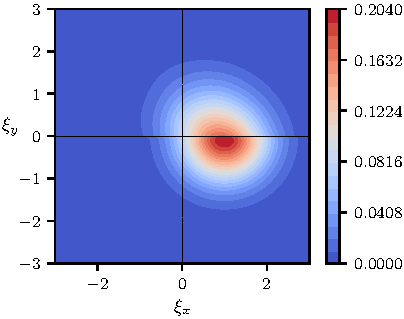
\includegraphics[width=\linewidth]{{{couette/kn0.1-boundary}}}
            \caption{Возле границы \(y=0.4990\)}
        \end{figure}
        \column{.55\textwidth}
        \begin{figure}
            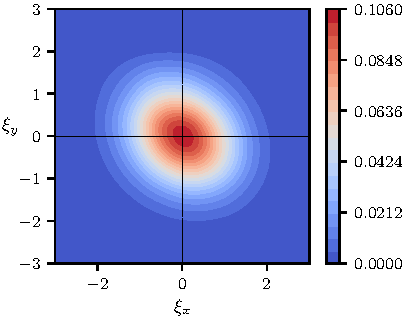
\includegraphics[width=\linewidth]{{{couette/kn0.1-center}}}
            \caption{Вблизи центра \(y=0.0082\)}
        \end{figure}
    \end{columns}
\end{frame}

\begin{frame}
    \frametitle{Функция распределения \(\Delta{v}=2\), срез \(\zeta_z=0.1665\)}
    \vspace{-20pt} \[ Kn=1 \] \vspace{-20pt}
    \begin{columns}
        \column{.55\textwidth}
        \begin{figure}
            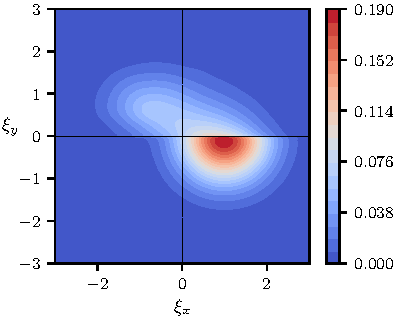
\includegraphics[width=\linewidth]{{{couette/kn1.0-boundary}}}
            \caption{Возле границы \(y=0.4929\)}
        \end{figure}
        \column{.55\textwidth}
        \begin{figure}
            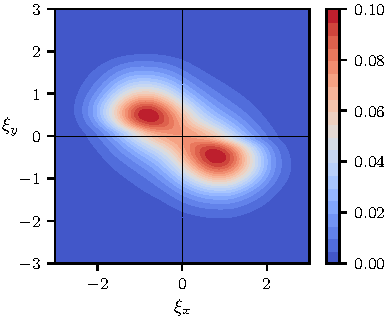
\includegraphics[width=\linewidth]{{{couette/kn1.0-center}}}
            \caption{Вблизи центра \(y=0.0083\)}
        \end{figure}
    \end{columns}
\end{frame}

\begin{frame}
    \frametitle{Функция распределения \(\Delta{v}=2\), срез \(\zeta_z=0.1665\)}
    \vspace{-20pt} \[ Kn=10 \] \vspace{-20pt}
    \begin{columns}
        \column{.55\textwidth}
        \begin{figure}
            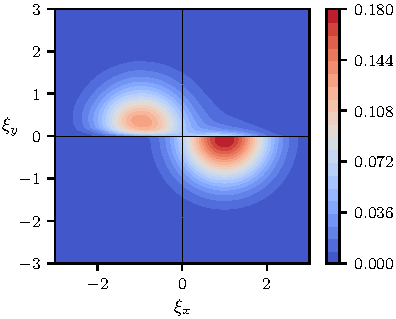
\includegraphics[width=\linewidth]{{{couette/kn10-boundary}}}
            \caption{Возле границы \(y=0.4917\)}
        \end{figure}
        \column{.55\textwidth}
        \begin{figure}
            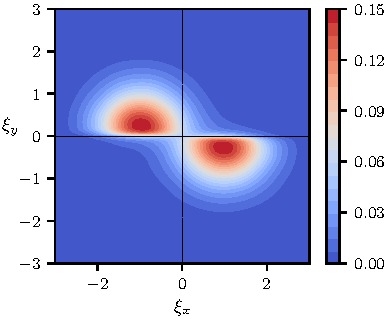
\includegraphics[width=\linewidth]{{{couette/kn10-center}}}
            \caption{Вблизи центра \(y=0.0083\)}
        \end{figure}
    \end{columns}
\end{frame}

\begin{frame}
    \frametitle{Профили сдвигового напряжения}
    \centering
    \includegraphics[width=0.9\linewidth]{couette/Pxy}
\end{frame}

\begin{frame}
    \frametitle{Профили продольной скорости}
    \centering
    \includegraphics[width=0.9\linewidth]{couette/vx}
\end{frame}

\begin{frame}
    \frametitle{Профили температуры}
    \centering
    \includegraphics[width=0.9\linewidth]{couette/tau}
\end{frame}

\begin{frame}
    \frametitle{Профили поперечного теплового потока}
    \centering
    \includegraphics[width=0.9\linewidth]{couette/qy}
\end{frame}

\begin{frame}
    \frametitle{Профили продольного теплового потока}
    \centering
    \includegraphics[width=0.9\linewidth]{couette/qx}
\end{frame}

\begin{frame}
    \frametitle{Профили давления}
    \centering
    \includegraphics[width=0.9\linewidth]{couette/P}
\end{frame}

\begin{frame}
    \frametitle{Профили \(P_{yy}\)}
    \centering
    \includegraphics[width=0.9\linewidth]{couette/Pyy}
\end{frame}

\begin{frame}
    \frametitle{Профили \(P_{xx}\)}
    \centering
    \includegraphics[width=0.9\linewidth]{couette/Pxx}
\end{frame}

\begin{frame}
    \frametitle{Профили \(P_{zz}\)}
    \centering
    \includegraphics[width=0.9\linewidth]{couette/Pzz}
\end{frame}

%%% vs Kn

\begin{frame}
    \frametitle{Зависимость сдвигового напряжения от \(\Kn\)}
    \vspace{-2pt}
    \centering\hspace{-1.5cm}
    \includegraphics[width=1.1\linewidth]{couette2/shear}
    \hspace{-1.5cm}
\end{frame}

\begin{frame}
    \frametitle{Зависимость продольной скорости от \(\Kn\)}
    \vspace{-2pt}
    \centering\hspace{-1.5cm}
    \includegraphics[width=1.1\linewidth]{couette2/flow}
    \hspace{-1.5cm}
\end{frame}

\begin{frame}
    \frametitle{Зависимость продольного теплового потока от \(\Kn\)}
    \vspace{-2pt}
    \centering\hspace{-1.5cm}
    \includegraphics[width=1.1\linewidth]{couette2/qflow}
    \hspace{-1.5cm}
\end{frame}

\begin{frame}
    \frametitle{Зависимость поперечного теплового потока от \(\Kn\)}
    \vspace{-2pt}
    \centering\hspace{-1.5cm}
    \includegraphics[width=1.1\linewidth]{couette2/qflowy}
    \hspace{-1.5cm}
\end{frame}

\begin{frame}
    \frametitle{Зависимость \(P_{zz}\) от \(\Kn\)}
    \vspace{-2pt}
    \centering\hspace{-1.5cm}
    \includegraphics[width=1.1\linewidth]{couette2/pzz}
    \hspace{-1.5cm}
\end{frame}

%%%%%%%%%%%%%%%%%%%%%%%%%%%%%%%%%%%%%%%%%%%%%%%%%%%%%%%%%%%%%%%%%%%
\begin{comment}

\subsection{Задача Соне--Бобылева}

\begin{frame}
    \frametitle{Задача Соне--Бобылева}
    \begin{columns}
        \column{.5\textwidth}
        \hspace{-10pt}\includegraphics{sone_bobylev/geometry}
        \column{.6\textwidth}
        \[ T_B = 1 - \frac{\cos(2\pi x)}{2}, \quad v_{Bi} = 0 \]
        \begin{itemize}
            \item \(\Kn\to0\) для модели БКВ и твёрдых сфер [Sone et al. 1996]
            \smallskip
            \item \(\Kn=\OO{1}\) для модели БКВ [Sone et al. 1996]
            \smallskip
            \item \(\Kn=\OO{1}\) для твёрдых сфер
        \end{itemize}
    \end{columns}
\end{frame}

\begin{frame}
    \frametitle{Изотермические линии в континуальном пределе}
    \begin{columns}
        \column{.55\textwidth}
        \begin{figure}
            \includegraphics[width=\linewidth]{sone_bobylev/heat-temp}
            \caption{уравнение теплопроводности}
        \end{figure}
        \column{.55\textwidth}
        \begin{figure}
            \includegraphics[width=\linewidth]{sone_bobylev/snif-0-temp}
            \caption{уравнения КГФ}
        \end{figure}
    \end{columns}
\end{frame}

\begin{frame}
    \frametitle{Поле скоростей в континуальном пределе}
    \begin{columns}
        \column{.55\textwidth}
        \begin{figure}
            \includegraphics[width=\linewidth]{sone_bobylev/snif-0-flow}
            \caption{уравнения КГФ со скольжением (\(b_2 = 0.64642\))}
        \end{figure}
        \column{.55\textwidth}
        \begin{figure}
            \includegraphics[width=\linewidth]{sone_bobylev/nonslip-0-flow}
            \caption{уравнение КГФ без скольжения (\(b_2 = 0\))}
        \end{figure}
    \end{columns}
\end{frame}

\begin{frame}
    \frametitle{Изотермические линии при \(\Kn=0.01\)}
    \begin{columns}
        \column{.55\textwidth}
        \begin{figure}
            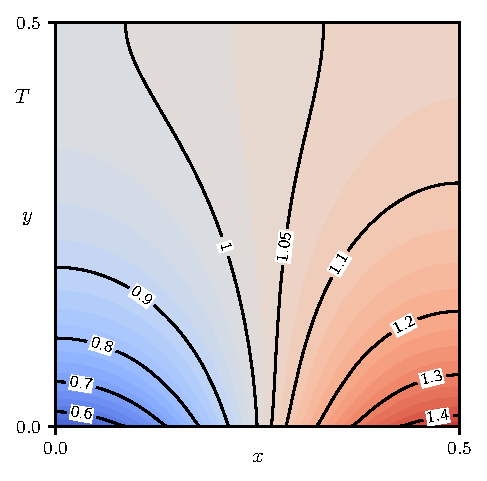
\includegraphics[width=\linewidth]{{{sone_bobylev/asym-0.01-temp}}}
            \caption{уравнения КГФ с учётом температурного скачка}
        \end{figure}
        \column{.55\textwidth}
        \begin{figure}
            \includegraphics[width=\linewidth]{{{sone_bobylev/data-0.01-temp}}}
            \caption{численное решение уравнения Больцмана}
        \end{figure}
    \end{columns}
\end{frame}

\begin{frame}
    \frametitle{Поле скоростей при \(\Kn=0.01\)}
    \begin{columns}
        \column{.55\textwidth}
        \begin{figure}
            \includegraphics[width=\linewidth]{{{sone_bobylev/asym-0.01-flow}}}
            \caption{уравнения КГФ с учётом температурного скачка}
        \end{figure}
        \column{.55\textwidth}
        \begin{figure}
            \includegraphics[width=\linewidth]{{{sone_bobylev/data-0.01-flow}}}
            \caption{численное решение уравнения Больцмана}
        \end{figure}
    \end{columns}
\end{frame}

\begin{frame}
    \frametitle{Зависимость температурного поля от \(\Kn\)}
    \centering
    \includegraphics[width=0.9\linewidth]{sone_bobylev/bottom_temp}
\end{frame}

\begin{frame}
    \frametitle{Зависимость скоростного поля от \(\Kn\)}
    \centering
    \includegraphics[width=0.9\linewidth]{sone_bobylev/top_temp}
\end{frame}

\begin{frame}
    \frametitle{Зависимость температурного поля от \(\Kn\)}
    \centering
    \includegraphics[width=0.9\linewidth]{sone_bobylev/bottom_flow}
\end{frame}

\begin{frame}
    \frametitle{Зависимость скоростного поля от \(\Kn\)}
    \centering
    \includegraphics[width=0.9\linewidth]{sone_bobylev/top_flow}
\end{frame}

\subsection{Течение между некоаксиальными цилиндрами}

\begin{frame}
    \frametitle{Поле скоростей в континуальном пределе}
    \centering
    \begin{figure}
    \begin{overprint}
        \onslide<1| handout:2>
            \[ T_1 = 1, \quad T_2 = 5.\]
            \hspace{-1cm}
            \includegraphics[width=1.15\linewidth]{noncoaxial/cylinder5}
        \onslide<2| handout:1>
            \[ T_1 = 5, \quad T_2 = 1.\]
            \hspace{-1cm}
            \includegraphics[width=1.15\linewidth]{noncoaxial/inverse5}
        \onslide<3| handout:0>
            \[ T_1 = 1, \quad T_2 = 50.\]
            \hspace{-1cm}
            \includegraphics[width=1.15\linewidth]{noncoaxial/cylinder50}
    \end{overprint}
    \hspace{-.5cm}
    \end{figure}
\end{frame}

\begin{frame}
    \frametitle{Зависимость поля скоростей от \(\tau = T_2-T_1\)}
    \centering
    \begin{columns}
        \column{.7\textwidth}
        \begin{figure}
            \includegraphics[width=\linewidth]{noncoaxial/U-tau-cylinders}
            \vspace{-.5cm}\caption{максимальное значение скорости}
        \end{figure}
        \column{.4\textwidth}
        \[ u_{i1} = \OO{\tau^3}, \quad \tau\to0, \]
        \[ u_{i1} = \OO{\tau^{3/2}}, \quad \tau\to\infty. \]
    \end{columns}
\end{frame}

\begin{frame}
    \frametitle{Зависимость действующей силы от \(\tau = T_2-T_1\)}
    \vspace{-.2cm}
    \[ p_0 \oint_S F_{x2}\dd{S} = \OO{\tau^2}. \]
    \vspace{-.7cm}
    \begin{columns}
        \column{.6\textwidth}
        \begin{figure}
            \includegraphics[width=\linewidth]{noncoaxial/F-tau-cylinders-inner}
            \vspace{-.5cm}\caption{внутренний цилиндр}
        \end{figure}
        \column{.6\textwidth}
        \begin{figure}
            \includegraphics[width=\linewidth]{noncoaxial/F-tau-cylinders-outer}
            \vspace{-.5cm}\caption{внешний цилиндр}
        \end{figure}
    \end{columns}
\end{frame}

\begin{frame}
    \frametitle{Зависимость действующей силы от расстояния между осями}
    \vspace{-.5cm}
    \[ p_0 \oint_S F_{x2}\dd{S} = \begin{cases}
        \OO{(1-d)^{-1}} & \quad\text{для cфер}, \\
        \OO{(1-d)^{-3/2}} & \quad\text{для цилиндров}, \\
        \end{cases} \quad d\to1. \]
    \vspace{-.7cm}
    \begin{columns}
        \column{.6\textwidth}
        \begin{figure}
            \includegraphics[width=\linewidth]{noncoaxial/forces}
        \end{figure}
        \column{.6\textwidth}
        \begin{figure}
            \includegraphics[width=\linewidth]{noncoaxial/forces-close}
        \end{figure}
    \end{columns}
\end{frame}

\begin{frame}
    \frametitle{Электростатическая аналогия}
    \begin{equation}
        p_0\oint_S F_{x2}\dd{S} = \pder[C]{d} \tau^2.
    \end{equation}
    \pause
    \vspace{10pt}

    Формулы для ёмкости [Smythe1968]:
    \begin{gather}
        C_\mathrm{cyl} \propto \frac1{\theta}, \\
        C_\mathrm{sph} \propto  \sum_{n=1}^\infty \frac{R_1 R_2 \sinh\theta} {R_2\sinh n\theta - R_1\sinh (n-1)\theta}, \\
        \cosh\theta = \frac{R_1^2 + R_2^2 - d^2}{2 R_1 R_2}.
    \end{gather}
\end{frame}


\begin{frame}
    \frametitle{Профили составляющих силу компонент}
    \begin{columns}
        \column{.6\textwidth}
        \begin{figure}
            \includegraphics[width=\linewidth]{noncoaxial/terms-cylinder-inner}
            \vspace{-.5cm}\caption{внутренний цилиндр}
        \end{figure}
        \column{.6\textwidth}
        \begin{figure}
            \includegraphics[width=\linewidth]{noncoaxial/terms-cylinder-outer}
            \vspace{-.5cm}\caption{внешний цилиндр}
        \end{figure}
    \end{columns}
\end{frame}

\end{comment}
%%%%%%%%%%%%%%%%%%%%%%%%%%%%%%%%%%%%%%%%%%%%%%%%%%%%%%%%%%%%%%%%%%%

\subsection{Течение между эллиптическими цилиндрами}

\begin{frame}
    \frametitle{Поле скоростей в континуальном пределе}
    \[ T_1 = 1, \quad T_2 = 5.\]
    \centering
    \hspace{-1cm}
    \includegraphics[width=1.1\linewidth]{elliptic/U}
    \hspace{-1cm}
\end{frame}

\begin{frame}
    \frametitle{Момент действующей силы в континуальном пределе}
    \begin{columns}
        \column{.55\textwidth}
        \begin{figure}
            \includegraphics[width=\linewidth]{elliptic/moment-beta}
            \caption{полный момент сил}
        \end{figure}
        \column{.55\textwidth}
        \begin{figure}
            \includegraphics[width=\linewidth]{elliptic/profiles}
            \caption{профиль удельного момента}
        \end{figure}
    \end{columns}
\end{frame}

\begin{frame}
    \frametitle{Поле скоростей при \(\Kn=0.02\) [Rogozin 2017]}
    \begin{figure}
        \hspace{-.5cm}
        \begin{overprint}
            \onslide<1| handout:3>
                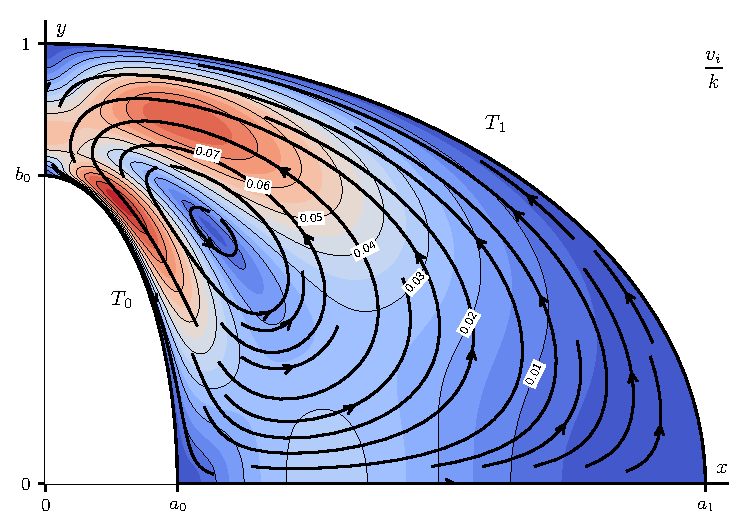
\includegraphics[width=\linewidth]{{{elliptic/kgf-0.02-flow}}}
                \vspace{-20pt}
                \caption{уравнения КГФ с граничными условиями ведущего порядка}
            \onslide<2| handout:2>
                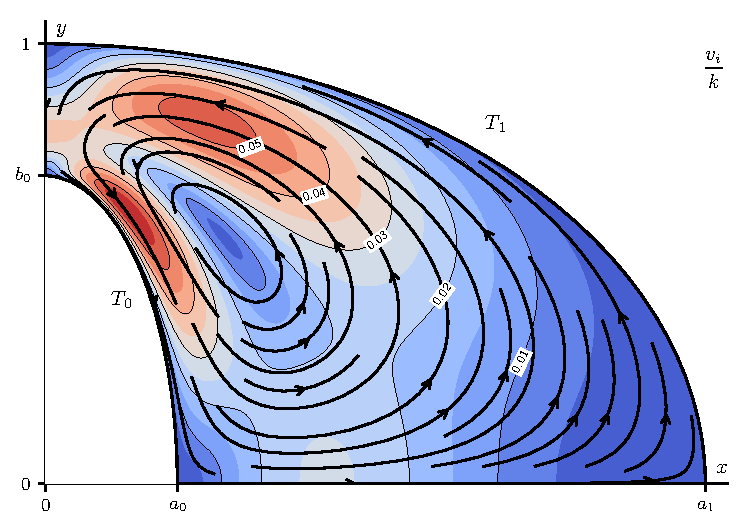
\includegraphics[width=\linewidth]{{{elliptic/first-0.02-flow}}}
                \vspace{-20pt}
                \caption{уравнения КГФ с граничными условиями первого порядка}
            \onslide<3| handout:1>
                \includegraphics[width=\linewidth]{{{elliptic/second-0.02-flow}}}
                \vspace{-20pt}
                \caption{уравнения КГФ с граничными условиями второго порядка}
            \onslide<4| handout:0>
                \includegraphics[width=\linewidth]{{{elliptic/kes-0.02-flow}}}
                \vspace{-20pt}
                \caption{численное решение уравнения Больцмана}
        \end{overprint}
    \end{figure}
\end{frame}

\end{document}
